% *********************************************************************
% © 2021-2022 Jeremy Sylvestre
%
% Permission is granted to copy, distribute and/or modify this document
% under the terms of the GNU Free Documentation License, Version 1.3 or
% any later version published by the Free Software Foundation; with no
% Invariant Sections, no Front-Cover Texts, and no Back-Cover Texts. A
% copy of the license is included in the appendix entitled “GNU Free
% Documentation License” that appears in the output document of this
% PreTeXt source code. All trademarks™ are the registered® marks of
% their respective owners.
%
% *********************************************************************

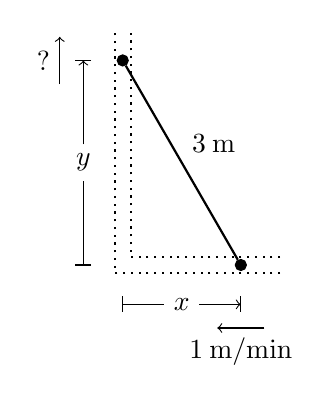
\begin{tikzpicture}
[
	closedpt/.style={circle,draw,fill,inner sep=0pt,minimum size=4pt},
	openpt/.style={circle,draw,inner sep=0pt,minimum size=4pt},
	scale=1
]

	\node[closedpt] at (1.5,0) (trail) {};
	\node[closedpt] at (0,2.598) (lead) {};

	\draw[thick] (trail) to node[above right] {$3\:\mathrm{m}$} (lead);

	\draw[thick,dotted] (2,0.1) -- (0.1,0.1) -- (0.1,3);
	\draw[thick,dotted] (2,-0.1) -- (-0.1,-0.1) -- (-0.1,3);

	\node at (0.75,-0.5) (x) {$x$};
	\draw[thin] (0,-0.4) -- (0,-0.6);
	\draw[thin] (1.5,-0.4) -- (1.5,-0.6);
	\draw[thin] (0,-0.5) -- (x);
	\draw[thin,->] (x) -- (1.5,-0.5);

	\node at (-0.5,1.299) (y) {$y$};
	\draw[thin] (-0.4,0) -- (-0.6,0);
	\draw[thin] (-0.4,2.598) -- (-0.6,2.598);
	\draw[thin] (-0.5,0) -- (y);
	\draw[thin,->] (y) -- (-0.5,2.598);

	\draw[->] (1.8,-0.8) -- node[below] {$1\:\mathrm{m}/\mathrm{min}$} (1.2,-0.8);
	\draw[->] (-0.8,2.298) -- node[left] {?} (-0.8,2.898);

\end{tikzpicture}
